% ---------- Titelblad Masterproef Faculteit Wetenschappen -----------
% Dit document is opgesteld voor compilatie met pdflatex.  Indien je
% wilt compileren met latex naar dvi/ps, dien je de figuren naar
% (e)ps-formaat om te zetten.
%                           -- december 2012
% -------------------------------------------------------------------
\RequirePackage{fix-cm}
\documentclass[12pt,a4paper,oneside]{book}

% --------------------- In te laden pakketten -----------------------
% Deze kan je eventueel toevoegen aan de pakketten die je al inlaadt
% als je dit titelblad integreert met de rest van thesis.
% -------------------------------------------------------------------
\usepackage{graphicx,xcolor,textpos}
\graphicspath{{images/}}

\usepackage{helvet}

\usepackage[linktoc=all]{hyperref}

\usepackage[dutch]{babel}

\usepackage{slashbox}


\usepackage{amsthm}
\theoremstyle{definition}
\newtheorem{exmp}{Voorbeeld}[section]

\usepackage{listings}



\newcommand{\quotes}[1]{``#1''}

% -------------------- Pagina-instellingen --------------------------
% Indien je deze wijzigt, zal het titelblad ook wijzigen.  Dit dien je
% dan manueel aan te passen.
% --------------------------------------------------------------------

\topmargin -10mm
\textwidth 160truemm
\textheight 240truemm
\oddsidemargin 0mm
\evensidemargin 0mm

% ------------------- textpos-instellingen ---------------------------
% Enkele andere instellingen voor het voorblad.
% --------------------------------------------------------------------

\definecolor{green}{RGB}{172,196,0}
\definecolor{bluetitle}{RGB}{29,141,176}
\definecolor{blueaff}{RGB}{0,0,128}
\definecolor{blueline}{RGB}{82,189,236}
\setlength{\TPHorizModule}{1mm}
\setlength{\TPVertModule}{1mm}

\begin{document}

% ---------------------- Voorblad ------------------------------------
% Vergeet niet de tekst aan te passen:
% - Titel en, indien van toepassing, ondertitel
%          voor eventuele formules in de titel of ondertitel
%          gebruik je  \form{$...$}
% - Je naam
% - Je (co)promotor, begeleider (indien van toepassing)
% - Je opleiding
% - Het academiejaar
% --------------------------------------------------------------------
\thispagestyle{empty}
\newcommand{\form}[1]{\scalebox{1.087}{\boldmath{#1}}}
\sffamily
%
\begin{textblock}{191}(-24,-11)
\colorbox{green}{\hspace{123mm}\ \parbox[c][18truemm]{68mm}{\textcolor{white}{FACULTEIT WETENSCHAPPEN}}}
\end{textblock}
%
\begin{textblock}{70}(-18,-19)
\textblockcolour{}
\includegraphics*[height=19.8truemm]{LogoKULeuven}
\end{textblock}
%
\begin{textblock}{160}(-6,63)
\textblockcolour{}
\vspace{-\parskip}
\flushleft
\fontsize{40}{42}\selectfont \textcolor{bluetitle}{Programmeren met Onzekerheid: Een Case Study}\\[1.5mm]
\fontsize{20}{22}\selectfont Ondertitel \form{$S=\pi r^2$\textsl{(facultatief)}}
\end{textblock}
%
\begin{textblock}{160}(8,153)
\textblockcolour{}
\vspace{-\parskip}
\flushright
\fontsize{14}{16}\selectfont \textbf{Sus VERWIMP}
\end{textblock}
%
\begin{textblock}{70}(-6,191)
\textblockcolour{}
\vspace{-\parskip}
\flushleft
Promotor: Prof. T. Schrijvers\\[-2pt]
\textcolor{blueaff}{Affiliatie \textsl{(facultatief)}}\\[5pt]
%Co-promotor: \textsl{(facultatief)}\\[-2pt]
%\textcolor{blueaff}{Affiliatie \textsl{(facultatief)}}\\[5pt]
Begeleider: \textsl{A. Vandenbroucke (facultatief)}\\[-2pt]
\textcolor{blueaff}{Affiliatie \textsl{(facultatief)}}\\
\end{textblock}
%
\begin{textblock}{160}(8,191)
\textblockcolour{}
\vspace{-\parskip}
\flushright
Proefschrift ingediend tot het\\[4.5pt]
behalen van de graad van\\[4.5pt]
Master of Science in\\[4.5pt]
Toegepaste Informatica\\
\end{textblock}
%
\begin{textblock}{160}(8,232)
\textblockcolour{}
\vspace{-\parskip}
\flushright
Academiejaar 2017-2018
\end{textblock}
%
\begin{textblock}{191}(-24,248)
{\color{blueline}\rule{550pt}{5.5pt}}
\end{textblock}
%
\vfill
\newpage
\thispagestyle{empty}
% Copyright statement
\textsf{\textcopyright} Copyright by KU Leuven
Zonder voorafgaande schriftelijke toestemming van zowel de promotor(en) als de auteur(s) is overnemen, kopiëren, gebruiken of realiseren van deze uitgave of gedeelten ervan verboden. Voor aanvragen tot of informatie i.v.m. het overnemen en/of gebruik en/of realisatie van gedeelten uit deze publicatie, wend u tot de KU Leuven, Faculteit Wetenschappen, Geel Huis, Kasteelpark Arenberg 11 bus 2100, 3001 Leuven (Heverlee), Telefoon +32 16 32 14 01.
\\\\
Voorafgaande schriftelijke toestemming van de promotor(en) is eveneens vereist voor het aanwenden van de in dit afstudeerwerk beschreven (originele) methoden, producten, schakelingen en programma’s voor industrieel of commercieel nut en voor de inzending van deze publicatie ter deelname aan wetenschappelijke prijzen of wedstrijden.

\vfill
\newpage

% Als je het titelblad wil integreren met de rest van je thesis,
% kan je hieronder verder.
% ----------------------- Eerste pagina's -------------------------
% Hier kan je inhoudsopgave, voorwoord en dergelijke kwijt.
% -----------------------------------------------------------------
\rmfamily
\setcounter{page}{0}
\pagenumbering{roman}
\frontmatter
\chapter{Voorwoord}
\chapter{Korte Samenvatting}
\chapter{Lijst van afkortingen en lijst van symbolen}
\tableofcontents


\newpage
% ----------------------- Eigenlijke thesis -----------------------
% Vanaf de inleiding/het eerste hoofdstuk.
% -----------------------------------------------------------------
\mainmatter
\setcounter{page}{0}
\pagenumbering{arabic}

\chapter{Inleiding}
De grote interesse in het redeneren met onzekerheid in Artifici\"{e}le Intelligentie resulteert in de ontwikkeling van verschillende programmeertalen. Deze talen worden probabilistische programmeertalen of PPL (Probabilistic Programming Language) genoemd. Een PPL heeft in grote lijnen 2 hoofddooelen:
\begin{itemize}
  \item Het modelleren van een wereld met onzekerheid.
  \item Het redeneren/infereren van vragen over deze wereld met behulp van dit model.
\end{itemize}
Voorheen was het zeer moeilijk als programmeur om werelden met onzekerheid te modelleren. Probabilistische problemen werden geprogrammeerd aan de hand van grafische modellen zoals onder andere bayesiaanse netwerken. Het redeneren over deze modellen gebeurde met inferentie methodes die speciaal werden opgesteld voor het gemodelleerde probleem. Dit zorgde ervoor dat code voor een model niet herbruikbaar was en elke inferentie methode opnieuw ge\"{i}mplementeerd moest worden voor elk probleem. Met de komst van PPL's zijn deze problemen opgelost. Elke PPL heeft zijn eigen manier van implementatie en wordt vaak ge\"{i}mplementeerd als extensie op een general-purpose programmeertaal. Dit zorgt ervoor dat een PPL expressiever wordt. Gebruikers van een PPL kunnen een probabilistisch probleem volledig specifieren in het model en de bestaande inferentie methodes gebruiken om te redeneren over dit probleem. De general-purpose programmeertaal zorgt voor het hergebruiken van bestaande libraries en modellen. Algemene inferentiealgoritmes worden eenmalig gemaakt voor deze PPL zodat deze werkt voor alle modellen. Veel van deze PPL’s streven naar een balans tussen performantie en expressiviteit. Het is belangrijk voor een PPL om problemen te kunnen modelleren en tegelijkertijd op een aanvaardbare tijd te kunnen redeneren over vragen over dit model.
\\\\
Sinds de laatste jaren zijn er veel verschillende PPL's beschikbaar zoals ProbLog2, Anglican,... De url \url{http://probabilistic-programming.org/wiki/Home} geeft een overzicht van de verschillende PPL's die momenteel beschikbaar zijn.
Omdat er zo veel PPL's beschikbaar zijn, is het niet altijd duidelijk wat de voordelen of nadelen ten opzichte van elkaar zijn. Verschillende van deze PPL's zijn in recente artikels vergeleken met elkaar op het vlak van eigenschappen en concepten van de taal \cite{plpconcepts}. Andere artikels vergelijken vorige iteraties van dezelfde taal of PPL's met hetzelfde programmeerparadigma (bvb. logische of functionele programmeren) \cite{plpinferencelearningwbf}. Het probleem bij deze vergelijkingen en evaluaties is dat er nooit evaluaties gedaan worden voor PPL's met een verschillend programmeerparadigma.
\\\\
In deze thesis ben ik van plan PPL's met verschillende programmeerparadigma zoals ProbLog2 en Anglican te vergelijken en evalueren. het is de bedoeling deze PPL's te evalueren ten opzichte van elkaar aan de hand van qualitatieve en quantitatieve criteria zoals: performantie, expressiviteit, geheugengebruik, uitbreidbaarheid, beschikbare tools, moeilijkheidsgraad,... Omdat het niet triviaal is om programmeertalen te vergelijken die totaal anders ge\"{i}mplementeerd zijn gebeurd de evaluatie aan de hand van een case study. De implementatie van deze case-study in ProbLog2 en Anglican vormt het vertrekpunt voor een vergelijking van deze twee programmeertalen op basis van de hogervernoemde criteria. Uiteindelijk zal deze thesis aantonen welke PPL het best presteert in welke criteria aan de hand van het opgegeven probleem.

\chapter{Achtergrond}
In deze sectie vindt u de nodige achtergrondinformatie om de rest van deze thesis te begrijpen.
\section{Redeneren met Onzekerheid}
Redeneren met onzekerheid is \'{e}\'{e}n van de invloedrijkste domeinen van Artifici\"{e}le Intelligentie. De reden hiervoor is omdat het universum van nature veel onzekerheid bevat. Denk aan de volgende punten:
\begin{itemize}
	\item Kennis (We kunnen niet alles van het toepassingsdomein weten.)
	\item Onvolledige modellen (verschijnselen die niet onder het model vallen)
	\item Sensoren (We kunnen de wereld enkel observeren met de tools die geen exacte resultaten geven.)
\end{itemize}
Er zijn 3 belangrijke kwesties in verband met het werken met onzekerheid:
\begin{itemize}
	\item Voorstellen van onzekerheid
	\item Redeneren met onzekerheid
	\item Leren aan de hand van onzekerheid
\end{itemize}
Het voorstellen van onzekerheid gebeurt in een model van een onzekerheidsprobleem. Een model is een weergave van een onzekerheidsprobleem waarbij iedere mogelijke wereld kan gesimuleerd worden (zie voorbeeld~\ref{exmp:faircoin}). Onzekerheidsproblemen zijn problemen waar er weinig of geen zekerheid is over de uitkomst van een actie.
\begin{exmp}
\label{exmp:faircoin}
Een voorbeeld van een onzekerheidsprobleem met weinig zekerheid is het tossen van een eerlijk muntstuk. Hier zijn we zeker dat als we het muntstuk tossen dat het 50\% kans heeft om te landen op kop of munt, maar er is geen zekerheid wat het resultaat is. De actie is hier het tossen van een munt. Deze actie heeft twee mogelijke resultaten, of twee mogelijke werelden: namelijk de wereld waar het muntstuk land op kop en de wereld waar het muntstuk land op munt. Bij een eerlijke munt is de kans dat de eerste wereld bestaat 50\% en de kans dat de tweede wereld 50\%. We weten pas wat het resultaat is als we het resultaat zien. Het resultaat van de actie verandert dan in een gegeven of bewijsmateriaal van het model.
\end{exmp}
\begin{exmp}
Een voorbeeld van een onzekerheidsprobleem met geen zekerheid is het tossen van een random muntstuk. Hier weten we niet of het een eerlijk muntstuk is of een muntstuk waar met geknoeid is. In dit onzekerheidsprobleem zijn er nog steeds twee mogelijke werelden die bestaan als de tos actie wordt uitgevoerd. Het verschil met het vorige voorbeeld is dat de munt nu een random munt is, dus de werelden die kunnen bestaan kunnen een andere kansverdeling hebben. Een onzekerheidsprobleem met geen zekerheid wordt zo gemodelleerd dat het model de kansverdeling leert van interpretaties, in dit geval de resultaten van alle tossen. Het leren van interpretaties wordt niet toegepast in deze thesis.
\end{exmp}
Bij het redeneren over het onzekerheidsprobleem gebruiken we een model waar we vragen kunnen over stellen. Een model modelleert alle mogelijke werelden die kunnen bestaan in het onzekerheidsprobleem. Bij het redeneren zijn we op zoek naar de kans dat de vraag die we stellen waar is in het onzekerheidsprobleem. Voorbeeld~\ref{exmp:inferentiaexample} is een simpel voorbeeld voor het tossen van een eerlijk muntstuk.
\begin{exmp}
\label{exmp:inferentiaexample}
We hebben een eerlijk muntstuk. Wat is de kans dat we na 3 keer tossen 3 keer kop verkrijgen. Hier weten we dat het muntstuk eerlijk is dus 50\% kans heeft om op kop of munt te landen. De kans dat we 3 keer tossen en 3 keer munt verkrijgen is dus:
\\\\
$P(c1=kop \& c2=kop \& c3=kop) = \frac{1}{2} * \frac{1}{2} * \frac{1}{2} = \frac{1}{8}$
\\\\
Stel dat we het resultaat van de eerste tos weten en deze op kop landt. Omdat we dit weten kunnen we dit aan het model meegeven als bewijsmateriaal van het model.
\\\\
c1 = kop
\\
$P(c1=kop \& c2=kop \& c3=kop) = 1 * \frac{1}{2} * \frac{1}{2} = \frac{1}{4}$
\end{exmp}
Voor kleine onzekerheidsproblemen als deze is dit nog makkelijk op te lossen met eenvoudige kans regels. Als het onzekerheidsprobleem groter is wordt het al moeilijker om dit te berekenen. In voorbeeld~\ref{exmp:inferentiaexamplealarm} stellen we een voorbeeld voor dat al moeilijker op te lossen is met simpele kans regels.
\begin{exmp}
\label{exmp:inferentiaexamplealarm}
Stel dat we in een huis wonen in een regio waar er 20\% kans is op een aardbeving en 70\% kans is op een inbraak in het huis. We installeren een alarm in het huis. Op de verpakking van het alarm staan de kansen dat het alarm afgaat:
\begin{itemize}
	\item 90\% van de tijd gaat het alarm af als er een inbraak en een aardbeving is.
	\item 80\% van de tijd gaat het alarm af als er een inbraak is.
	\item 10\% van de tijd gaat het alarm af als er een aardbeving is.
	\item Als er geen inbraak of aardbeving is gaat het alarm niet af.
\end{itemize} 
Stel dat we het alarm horen afgaan. Wat is de kans dat er een aardbeving is als het alarm afgaat?
\end{exmp}
Elementen in het onzekerheidsprobleem die onderheven zijn aan kansen noemen we variabelen. In voorbeeld~\ref{exmp:inferentiaexamplealarm} zijn de variabelen:
\begin{itemize}
	\item Aardbeving
	\item Inbraak
	\item Alarm
\end{itemize}
Aardbeving en Inbraak hebben niets met elkaar te maken en als we iets weten over het \'{e}\'{e}n zorgt er niet voor dat we meer weten over het andere. Dit wilt zeggen dat deze variabelen conditioneel onafhankelijk zijn van elkaar. Alarm is conditioneel afhankelijk van Inbraak en Aardbeving. Als we weten dat er inbraak is kunnen we zeggen dat de kans dat het alarm afgaat vergroot. Hetzelfde gebeurd als er een aardbeving is.
\\\\
Dit probleem kunnen we visueel illustreren met een bayesiaans netwerk. Een bayesiaans netwerk illustreert alle variabelen van een onzekerheidsprobleem in cirkels en de pijlen tussen de cirkels stellen de afhankelijkheid van een variabele ten opzichte van een andere variabele voor. Figuur~\ref{figure:alarmearthquakeburglary} is een voorbeeld van een bayesiaans netwerk voor voorbeeld~\ref{exmp:inferentiaexamplealarm}. 
\begin{figure}
	\centering
	\includegraphics[height=60truemm]{alarm\string_earthquake\string_burglary}
	\caption{Bayesiaans netwerk van een onzekerheidsprobleem. Alarm is conditioneel afhankelijk van Inbraak en Aardbeving.}
	\label{figure:alarmearthquakeburglary}
\end{figure}
\\\\
Om het onzekerheidsprobleem uit voorbeeld~\ref{exmp:inferentiaexamplealarm} op te lossen maken we gebruik van de regel van Bayes.
\begin{equation} 
	\label{eq:bayesrule}
	P(Hypothese|Bewijs) = \frac{P(Bewijs|Hypothese)P(Hypothese)}{P(Bewijs)}
\end{equation}
Als we de benamingen van figuur~\ref{figure:alarmearthquakeburglary} gebruiken wordt dit:
\begin{equation} 
	\label{eq:bayesrule}
	P(AA=true|A=true) = \frac{P(A=true|AA=true)P(AA=true)}{P(A=true)}
\end{equation}
De regel van Bayes geeft de kans dat een hypothese waar is in het model waar er al dan niet bewijsmateriaal is dat influentie heeft op de kans dat de hypothese waar is. Meer informatie over bayesiaanse netwerken en het redeneren over deze netwerken in het boek \quotes{Bayesian Reasoning and Machine Learning} \cite{barberBRML2012}. 
\\\\
PPL's berekenen hetzelfde aan de hand van het inferentieproces dat de taal implementeert. Hoe ze dit doen verschilt voor elke PPL en wordt duidelijk uitgelegd in secties~\ref{subsubsec:inferentieProbLog2} en ~\ref{subsubsec:InferentieAnglican}. Het berekenen van de inferentie is een zeer krachtig, maar een zeer rekenintensief proces. Veel PPL's zoeken een balans tussen hoe efficient ze inferentie kunnen berekenen en welke problemen ze kunnen modelleren (hoe expressief de taal is).

\section{Probabilistische Programmeertalen}
Probabilistische programmeertalen (of PPL's van Probabilistic Programming Languages) zijn programmeertalen met 2 hoofddoelen:
\begin{itemize}
  \item Het modelleren van een wereld met onzekerheid.
  \item Het redeneren/infereren van vragen over deze wereld met behulp van dit model.
\end{itemize}
PPL's worden meestal ge\"{i}mplementeerd als extensie op bestaande general-purpose programmeertalen. PPL's zoals Anglican en Church zijn gebasseerd op een dialect van LISP (een functionele programmeertaal). ProbLog2 en PRISM zijn gebasseerd op Prolog (een logische programmeertaal). Voor sommige talen zoals Stan is een speciale taal ontwikkeld die niet gebasseerd is op een bestaande programmeertaal.
Deze thesis behandelt 2 PPL's, namelijk: ProbLog2 en Anglican. Secties~\ref{sec:ProbLog2} en~\ref{sec:Anglican} geven meer informatie over deze twee PPL's en hoe het modelleer- en inferentieproces werkt.
\subsection{ProbLog2}
\label{sec:ProbLog2}
ProbLog2 is een PPL gebaseerd op de programmeertaal Prolog. De volgende secties~\ref{subsubsec:ModellereninProbLog2} en~\ref{subsubsec:inferentieProbLog2} geven meer informatie over het modelleer- en inferentieproces. De volgende onderwerpen komen aan bod in sectie~\ref{subsubsec:ModellereninProbLog2}:
\begin{itemize}
	\item Syntax van een ProbLog programma
	\item Annotated Disjunction
	\item Flexibele kansen
\end{itemize} 
De volgende onderwerpen komen aan bod in sectie~\ref{subsubsec:inferentieProbLog2}:
\begin{itemize}
	\item Exacte inferentie
	\item benaderende inferentie
	\item inferentieproces voor exacte en benaderende inferentie
	\item stochastische memoisatie
	\item inferentieproces manipuleren met Python
\end{itemize} 
\subsubsection{Modelleren in ProbLog2}
\label{subsubsec:ModellereninProbLog2}
Een ProbLog2 programma bestaat uit 3 delen:
\begin{itemize}
	\item Een verzameling van gegronde probabilistische feiten
	\item Een logisch programma (verzameling van niet probabilistische regels)
	\item vragen en bewijsmateriaal over het model
\end{itemize}
een gegrond probabilistisch feit ziet er uit als \lstinline{p::f}. p is de kans dat het feit f waar is in het model. Het is ook mogelijk om gegronde probabilistische feiten volgens te schrijven als \lstinline{p::f(X1,X2,...,Xn) :- body}. Het is belangrijk dat body het domein definieert van de variabelen X1, X2,..., Xn.
\\\\
Een logisch programma bestaan uit niet probabilistische regels. Deze regels kunnen gebruik maken van probabilistische feiten.
\\\\
Vragen over het model komen in de vorm van \lstinline{query(f)} en bewijsmateriaal van het model komt in de vorm van \lstinline{evidence(f,Boolean)}. \lstinline{query(f)} vraagt aan ProbLog wat de kans is dat de regel f waar is in het model. f is een query atoom van het model. \lstinline{evidence(f,Boolean)} geeft bewijs dat regel f waar is of niet waar is in het model naar gelang de booleanse waarde die meegegeven wordt.
\\\\
Als we het onzekerheidsprobleem met het alarm en de aardbeving en de inbraak van voorbeeld~\ref{exmp:inferentiaexamplealarm} willen schrijven in ProbLog ziet het er als volgt uit:
\begin{lstlisting}
0.7::burglary.
0.2::earthquake.
0.9::p_alarm1.
0.8::p_alarm2.
0.1::p_alarm3.

alarm :- burglary, earthquake, p_alarm1.
alarm :- burglary, \+earthquake, p_alarm2.
alarm :- \+burglary, earthquake, p_alarm3.

evidence(alarm,true).
query(earthquake).
\end{lstlisting}
In bovenstaande code is het feit \lstinline{burglary}, \lstinline{earthquake}, \lstinline{p_alarm1},\lstinline{p_alarm2} en \lstinline{p_alarm3} geannotteerd met een kans. Dit zijn gegronde probabilistische feiten. \lstinline{0.7::burglary.} moet gelezen worden als: \quotes{er is 70\% kans dat inbraak waar is in het model}, Dit is analoog voor \lstinline{earthquake}, \lstinline{p_alarm1},\lstinline{p_alarm2} en \lstinline{p_alarm3}. Het feit \lstinline{alarm} is ook een gegrond probabilistisch feit maar deze is afgeleid van andere gegronde probabilistische feiten. Als de body van een afgeleid gegrond probabilistisch feit niet waar is, is het feit ook niet waar.
\\\\
We geven het model mee dat het alarm is afgegaan aan de hand van bewijsmateriaal (\lstinline{evidence(alarm,true).}). Daarna vragen we aan het model wat de kans is dat er een aardbeving is (\lstinline{query(earthquake).}).
\\\\
In de bovenstaande code maken we gebruik van gegronde probabilistische feiten zoals \lstinline{p_alarm1}, \lstinline{p_alarm2} en \lstinline{p_alarm3} om de kansen te bepalen dat het alarm afgaat bij bepaalde situaties zoals: \quotes{90\% kans dat het alarm afgaat als er een inbraak en een aardbeving is.}. Aan de hand van geannoteerde disjunctie kunnen we dit op een overzichtelijke manier schrijven. De code word dan:
\begin{lstlisting}
0.7::burglary.
0.2::earthquake.

0.9::alarm :- burglary, earthquake.
0.8::alarm :- burglary, \+earthquake.
0.1::alarm :- \+burglary, earthquake.

evidence(alarm,true).
query(earthquake).
\end{lstlisting}
geannoteerde disjunctie wordt ook gebruikt voor de kansverdeling te bepalen voor variabelen met een groter domein. In bovenstaande code is \lstinline{earthquake} terwijl waar of niet waar in het model. Als we dit willen uitbreiden naar 1\% kans op een zware aardbeving, 19\% kans op een lichte aardbeving en 80\% kans op geen aardbeving maken we gebruik van geannoteerde disjunctie. De code wordt dan:
\begin{lstlisting}
0.7::burglary.
0.01::earthquake(heavy); 0.19::earthquake(mild); 0.8::earthquake(none).

0.90::alarm :-   burglary, earthquake(heavy).
0.85::alarm :-   burglary, earthquake(mild).
0.80::alarm :-   burglary, earthquake(none).
0.10::alarm :- \+burglary, earthquake(mild).
0.30::alarm :- \+burglary, earthquake(heavy).

evidence(alarm,true).
query(earthquake(_)).
\end{lstlisting}
De puntkomma tussen de feiten \lstinline{earthquake} wilt zeggen dat er terwijl \lstinline{earthquake(heavy)}, \lstinline{earthquake(mild)} of \lstinline{earthquake(none)} waar is in het model maar nooit 2 van deze feiten.
\\\\
Stel dat de staat van het alarm degradeerd met de jaren en de kans dat het alarm afgaat vermindert met het aantal jaar dat het oud is. Dit kunnen we oplossen aan de hand van flexibele kansen. Flexibele kansen worden gebruikt als de kans dat een gegrond probabilistisch feit afhangt van andere waarden. De volgende code geeft een voorbeeld van een alarm systeem dat degradeerd met de jaren:
\begin{lstlisting}
0.7::burglary.
0.01::earthquake(heavy); 0.19::earthquake(mild); 0.8::earthquake(none).

P::alarm(Old) :- P is 0.90 - (Old / 100),   burglary, earthquake(heavy).
P::alarm(Old) :- P is 0.85 - (Old / 100),   burglary, earthquake(mild).
P::alarm(Old) :- P is 0.80 - (Old / 100),   burglary, earthquake(none).
P::alarm(Old) :- P is 0.10 - (Old / 100), \+burglary, earthquake(mild).
P::alarm(Old) :- P is 0.30 - (Old / 100), \+burglary, earthquake(heavy).

evidence(alarm(10),true).
query(earthquake(_)).
\end{lstlisting}
De combinatie van deze regels en het logisch programmeer systeem Prolog geeft ons de mogelijkheid om zeer uitgebreide onzekerheidsproblemen te modelleren. We kunnen vragen stellen aan deze modellen en deze vragen aan de hand van de inferentie machine van ProbLog2 oplossen. De volgende sectie~\ref{subsubsec:inferentieProbLog2} legt uit hoe deze vragen worden opgelost in ProbLog2.
\subsubsection{Inferentie}
\label{subsubsec:inferentieProbLog2}
De ProbLog2 inferentie machine kan verschillende inferentie taken oplossen, namelijk:
\begin{itemize}
	\item Marginale kansverdeling (MARG, Marginal)
	\item Meest waarschijnlijke verklaring (MPE, Most Probable Explenation)
	\item Leren van interpretaties
\end{itemize}
Deze thesis maakt enkel gebruik van het berekenen van de MARG.
\\\\
ProbLog2 kan de exacte en benaderende MARG berekenen van alle query atomen van het model. De exacte inferentie berekent de exacte kans dat een query atoom waar is in het model rekening houdend met alle mogelijke werelden die kunnen bestaan in het model. Benaderende inferentie maakt gebruik van X aantal samples om de MARG van een query atoom te berekenen. X is hier een vrije keuze. Elke sample berekent de kans dat een query atoom waar is voor \'{e}\'{e}n mogelijke wereld van het model. Als we gebruik maken van een groot aantal samples convergeert de benaderende MARG naar de exacte MARG. Dit komt een groot aantal samples ervoor zorgt dat de kans groot is dat alle mogelijke werelden in het model gesampled worden.
\\\\
Het inferentieproces voor het berekenen van de MARG in ProbLog2 maakt gebruik van een proces genaamd kennis compilatie (knowledge compilation). Het kennis compilatie proces volgt een aantal chronologische stappen. De volgende stappen zijn hetzelfde voor exacte en benaderende inferentie.
\begin{enumerate}
	\item ProbLog2 genereert een lijst van de query atomen en bewijsmateriaal van het ProbLog2 programma.
	\item Aan de hand van de query atomen wordt het ProbLog2 programma geconverteerd naar een ground programma.
	\item Het ground programma wordt geconverteerd naar booleaans gewogen formules.
\end{enumerate}
Door gebruik te maken van de booleaans gewogen formules kunnen we gebruik maken van wel gekende algoritmes. het berekenen van de exacte MARG gebeurd door de booleaanse gewogen formules te converteren naar een rekenkring zoals een \quotes{deterministic, decomposable negation normal form (d-DNNF)} of een \quotes{Binary decision diagram (BDD)}. De exacte inferentie wordt berekent door \quotes{Weighted Model Counting (WMC)} uit te voeren op de rekenkring. De rekenkring zorgt ervoor dat WMC met een aanvaardbare tijdcomplexiteit uitgevoerd kan worden.
\\\\
Benaderende inferentie wordt berekent aan de hand van een sampling techniek genaamd MC-SAT. Voor de ge\"{i}nteresseerde is er het artikel~\cite{plpinferencelearningwbf}. Dit artikel gaat dieper in op de verschillende stappen voor het berekenen van exacte en benaderende inferentie in ProbLog2. Voor deze thesis is het genoeg om te weten welke stappen er worden uitgevoerd tijdens het inferentieproces. Sectie~\ref{sec:evaluatieProbLog2} vertelt meer over de performantie van de verschillende stappen in het inferentieproces.
\\\\
Het ProbLog2 systeem kan gebruikt worden als een stand-alone tool of via Python. Via Python kan elke stap van het inferentieproces gemanipuleert worden. In sectie~\ref{sec:evaluatieProbLog2} staan verschillende voorbeelden waarom het gebruik maken van Python het inferentieproces kan versnellen voor de case study voorgesteld in sectie~\ref{subsec:uitwerkingSpel}.
\subsection{Anglican}
\label{sec:Anglican}
\subsubsection{Modelleren in Anglican}
\label{subsubsec:ModellerenInAnglican}
\subsubsection{Inferentie}
\label{subsubsec:InferentieAnglican}


\chapter{Uitwerking}
\section{Probleem verzinnen}
\label{sec:uitwerkingProblem}
Als onzekerheidsprobleem heb ik gekozen om een spel te modelleren dat onderheven is aan probabilistische aspecten. Om het spel te spelen heb ik 4 spelstrategiën ontwikkeld die elks ook onderheven zijn aan probabilistische aspecten.
\subsection{Spel}
\label{subsec:uitwerkingSpel}
Het spel bestaat uit een bord van 10 op 10 blokken. Wanneer het spel gestart wordt krijgen de blokken een random kleur toegewezen maar er kunnen geen 3 van dezelfde blokken op een rij staan (enkel verticaal en horizontaal). Er zijn 4 kleuren in totaal: rood, groen, geel, blauw. In figuur~\ref{figure:initialboard} ziet u een voorbeeld van een initi\"{e}el bord.
\begin{figure}
	\centering
	\includegraphics[height=60truemm]{grid\string_10x10\string_colors}
	\caption{voorbeeld van een initi\"{e}el bord}
	\label{figure:initialboard}
\end{figure}
\\\\
De speler kan op elk van de blokken op het bord drukken. Als de speler op een blok drukt verandert deze van kleur. De kleur waar de blok in veranderd hangt af van de probabilistische distributie. Om het simpel te houden gebruik ik hier een uniforme distributie:

\renewcommand{\arraystretch}{2}
\begin{table}
	\begin{center}
		\begin{tabular}{|c||*{4}{c|}}\hline
			\backslashbox{\textbf{Kleur blok}}{\textbf{Verandert in}}
			&\makebox[3em]{\textbf{Rood}}&\makebox[3em]{\textbf{Groen}}&\makebox[3em]{\textbf{Blauw}}&\makebox[3em]{\textbf{Geel}}\\\hline\hline
			\textbf{Rood}&0&$\frac{1}{3}$&$\frac{1}{3}$&$\frac{1}{3}$\\[2pt]\hline
			\textbf{Groen} &$\frac{1}{3}$&0&$\frac{1}{3}$&$\frac{1}{3}$\\[2pt]\hline
			\textbf{Blauw} &$\frac{1}{3}$&$\frac{1}{3}$&0&$\frac{1}{3}$\\[2ex]\hline
			\textbf{Geel} &$\frac{1}{3}$&$\frac{1}{3}$&$\frac{1}{3}$&0\\[2ex]\hline
		\end{tabular}
		\caption{\label{tab:changecolordistribution}Probabilistische distributie voor het veranderen van kleuren.}		
	\end{center}	
\end{table}
\renewcommand{\arraystretch}{1}

In woorden betekent dit dat als er op een rode blok wordt gedrukt er 1/3 kans is dat deze blok in een groene verandert, 1/3 kans in een blauwe verandert en 1/3 kans in een gele verandert. Voor een groene, blauwe en gele blok is dit analoog.
\\\\
Als er drie of meer blokken van dezelfde kleur ofwel horizontaal naast elkaar liggen ofwel verticaal naast elkaar liggen verdwijnen ze en dit levert punten op. De blokken die zich boven de verdwenen blokken bevinden vallen naar beneden tot ze op een andere blok belanden ofwel op de bodem van het spelbord belanden. Voor elke blok die verwijderd wordt krijgt de speler 1 punt. De bedoeling van het spel is om in 5 beurten zoveel mogelijk punten te behalen waarin de speler in elke beurt 1 blok van kleur mag veranderen. De beurt eindigt wanneer er geen 3 blokken van dezelfde kleur meer op een rij staan. In figuur 3 ziet u het verloop van een beurt in een 10x10 bord.
\begin{figure}
	\centering
	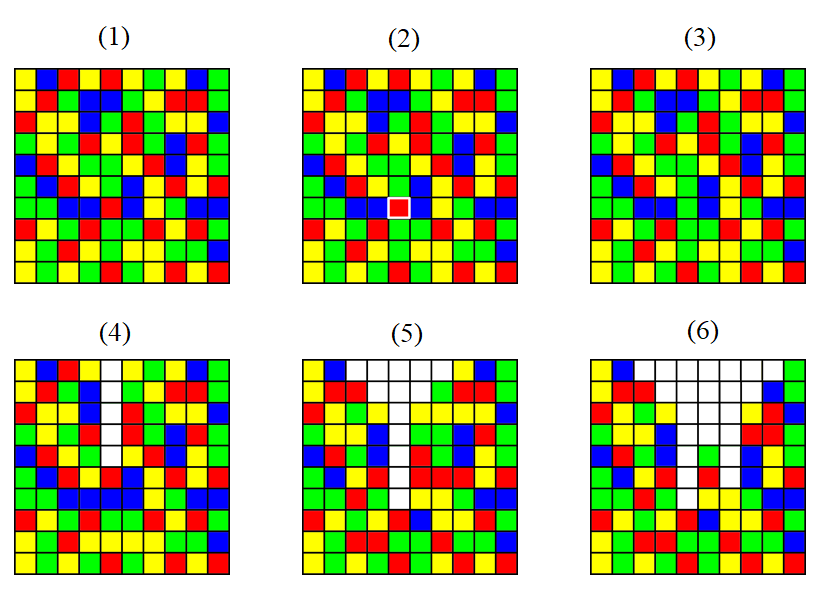
\includegraphics[height=80truemm]{turn}
	\caption{er wordt een blok gekozen om op te drukken, in dit geval een rode blok. De blok verandert met een 1/3 kans in een groene blok. Omdat er meer als 2 blokken van dezeflde kleur op een rij staan worden deze verwijderd en de bovenstaande blokken vallen naar beneden. Dit wordt herhaald tot er niet meer als 2 blokken van dezelfde kleur op een rij staan}
	\label{figure:initialboard}
\end{figure}
\subsection{Strategi\"{e}n}
Ik heb 4 strategiën ontwikkeld om het spel te spelen.
\begin{itemize}
	\item Uniforme strategie
	\item Kleuren ratio strategie
	\item Mogelijke score strategie
	\item Gewogen score strategie
\end{itemize}
Deze strategiën kunnen gebruikt worden om het spel te spelen op een bepaalde wijze. Elke strategie kiest altijd 1 blok uit de mogelijke blokken die beschikbaar zijn. Welk blok dit is hangt van de strategie af.

\subsubsection{Uniforme strategie}
Als de uniforme strategie wordt toegepast is de kans dat een blok gekozen wordt uniform voor elk blok in het spelbord. Voor een 10x10 bord is de kans dat een blok wordt gekozen . In figuur 4 zien we alle mogelijke keuzes die de uniforme strategie kan kiezen in het gegeven bord.
\begin{figure}
	\centering
	\includegraphics[height=70truemm]{uniform\string_strategy}
	\caption{In de uniforme strategie kunnen alle blokken gekozen worden met een uniforme kans verdeling. De kans is 1/100 voor elke blok in dit geval}
	\label{figure:initialboard}
\end{figure}

\subsubsection{Kleuren ratio strategie}
Voor de kleuren ratio strategie worden eerst alle blokken met dezelfde kleur opgeteld. Uit de kleur met het minst aantal blokken wordt uniform een blok gekozen. In figuur 5 zien we dat de blauwe blokken in de minderheid zijn. De strategie zorgt ervoor dat er uniform een blauwe blok wordt gekozen.
\begin{figure}
	\centering
	\includegraphics[height=70truemm]{color\string_ratio\string_strategy}
	\caption{In bovenstaande figuur is de kleuren ratio voor de blauwe blokken het minst. Hier wordt uniform een blauwe blok gekozen met een 1/17 kans voor elke blok}
	\label{figure:initialboard}
\end{figure}

\subsubsection{Mogelijke score strategie}
In de mogelijke score strategie wordt voor elke blok apart nagegaan of deze een mogelijke score kan hebben. Een blok kan een mogelijke score hebben als deze blok kan veranderen in een kleur die een score oplevert. In figuur 6 ziet u alle blokken aangeduid die een mogelijke score kunnen opleveren. Er wordt 1 blok uit deze blokken gekozen met een uniforme kansverdeling.
\begin{figure}
	\centering
	\includegraphics[height=70truemm]{possible\string_score\string_strategy}
	\caption{In een mogelijke score strategie wordt er uniform een blok gekozen uit alle blokken met een mogelijke score. In dit geval zijn er 48 blokken met een mogelijke score dus de kansverdeling is 1/48 voor elke blok}
	\label{figure:initialboard}
\end{figure}
\subsubsection{Gewogen score strategie}
De gewogen score strategie is een uitbreiding op de mogelijke score strategie waar we niet enkel naar de mogelijke score zien, maar naar de gewogen score. Elke blok kan veranderen van kleur aan de hand van een kansverdeling. De gewogen score strategie houdt rekening met deze kansverdeling. De gewogen score wordt berekend aan de hand van de score als een blok in Rood/Groen/Blauw/Geel verandert gewogen met de kans dat de blok verandert in Rood/Groen/Blauw/Geel.

\chapter{Evaluatie}
\label{ch:evaluatie}
\section{ProbLog2}
\label{sec:evaluatieProbLog2}
\section{Anglican}
\label{sec:evaluatieAnglican}
\section{ProbLog2 - Anglican}
\label{sec:evaluatieProbLog2Anglican}

\chapter{Conclusie}
\section{Toekomstig werk}

\bibliographystyle{plain}
\bibliography{./biblio}

\newpage
% ----------------------- Achterblad ------------------------------
% Vergeet niet de tekst aan te passen:
% - Afdeling
% - Adres van de afdeling
% - Telefoon en faxnummer
% -----------------------------------------------------------------
\thispagestyle{empty}
\sffamily
%
\begin{textblock}{191}(113,-11)
{\color{blueline}\rule{160pt}{5.5pt}}
\end{textblock}
%
\begin{textblock}{191}(168,-11)
{\color{blueline}\rule{5.5pt}{59pt}}
\end{textblock}
%
\begin{textblock}{183}(-24,-11)
\textblockcolour{}
\flushright
\fontsize{7}{7.5}\selectfont
\textbf{Faculteit Computerwetenschappen}\\
Geel Huis, Kasteelpark Arenberg 11 bus 2100\\
3001 LEUVEN, BELGI\"{E}\\
tel. + 32 16 32 14 01\\
%fax + 32 16 00 00 00\\
www.kuleuven.be\\
\end{textblock}
%
\begin{textblock}{191}(154,-7)
\textblockcolour{}
\includegraphics*[height=16.5truemm]{sedes}
\end{textblock}
%
\begin{textblock}{191}(-20,235)
{\color{bluetitle}\rule{544pt}{55pt}}
\end{textblock}
\end{document}